\chapter{Massaspectrometrie en atoomspectroscopie}\label{ch:b2:mass-spec-atomic}

Vuurwerk kleurt rood met strontiumzouten, groen met bariumzouten, geel met natrium: een vlam zet
atomen om in licht met kleuren die ze identificeren. Een massaspectrometer, bescheidener van uiterlijk,
weegt afzonderlijke moleculen, sorteert ze volgens hun isotopen en breekt ze in stukken waarvan de massa's vertellen
hoe ze gebouwd waren. Beide technieken beantwoorden de vraag ``wat zit er in dit monster, en hoeveel?''
uitgaande van zeer kleine hoeveelheden, de eerste voor moleculen, de tweede voor elementen.

\begin{omfigure}

\includegraphics[width=0.58\linewidth]{images/book3/ai/b2-32-fireworks.jpg}

{\small Vuurwerk boven een rivier (illustratie). Het geel van natrium is het licht van zijn atomen; het
diepe rood en groen komen grotendeels van kleine moleculen van strontium en barium die in de vlam gevormd worden.}
\end{omfigure}

\begin{recall}
Het schoolboek: isotopen en hun abundanties. Het deel van jaar~1: energieniveaus en
spectraallijnen, absorbantie en de wet van Beer--Lambert, carbokationen en radicalen, de onverzadigingsgraad.
\Cref{ch:b2:chromatography}: \omterm{def:b2:chromatography:techniques}{gaschromatografie}, die vaak een massaspectrometer voedt.
\end{recall}

\section{De massaspectrometer}

\begin{definition}[Massaspectrometrie]\label{def:b2:mass-spec-atomic:spectrum}
\emph{Massaspectrometrie}\index{massaspectrometrie} zet de moleculen van een monster om in gasvormige ionen,
scheidt de ionen volgens hun \emph{massa-ladingsverhouding}\index{massa-ladingsverhouding} $m/z$
(de massa in atomaire massa-eenheden gedeeld door het aantal ladingen) en telt ze. Het
\emph{massaspectrum}\index{massaspectrum} zet de abundantie van de ionen uit tegen $m/z$, meestal als
relatieve intensiteiten; zijn intenste piek, op 100 gezet, is de \emph{basispiek}\index{basispiek}.
\end{definition}

Een spectrometer heeft drie delen. De bron maakt ionen. Bij elektronionisatie (EI) kruist de damp van het
monster een bundel elektronen van \qty{70}{eV}, die een elektron uit de moleculen slaan en ze
met een overmaat energie achterlaten, zodat veel ervan uiteenvallen. Bij elektrospray-ionisatie (ESI) wordt een oplossing
verneveld uit een geladen naald; terwijl de druppeltjes verdampen, verlaten moleculen ze met een extra proton
(of een natriumion), intact: de methode bij uitstek voor grote, kwetsbare moleculen. De analysator sorteert daarna
de ionen, en een detector telt ze.

\begin{omfigure}
\begin{tikzpicture}[x=1cm, y=1cm]
\draw[black!70, fill=omDef!10, rounded corners=2pt] (0,-0.6) rectangle (1.6,0.6);
\node[font=\small, align=center] at (0.8,0) {ionen-\\bron};
\draw[black!70] (2.0,-0.7) -- (2.0,0.7); \draw[black!70] (2.4,-0.7) -- (2.4,0.7);
\node[font=\footnotesize] at (2.2,1.0) {roosters, $U$};
\draw[black!70] (2.6,-0.5) rectangle (8.4,0.5);
\node[font=\small] at (5.6,0.8) {veldvrije vluchtbuis, lengte $L$};
\draw[black!70, fill=black!15] (8.5,-0.6) rectangle (8.8,0.6);
\node[font=\small, align=center] at (9.6,0) {detector};
\foreach \x/\c in {3.4/omThm, 4.6/omDef, 6.3/omMeth}{\fill[\c] (\x,0) circle (0.1);}
\draw[->, thick] (6.6,0) -- (7.4,0);
\node[font=\footnotesize, align=center] at (5.5,-0.85) {lichte ionen voorop, zware achteraan};
\end{tikzpicture}
\par\vspace{4pt}

{\small Een vluchttijdanalysator (schematisch). Ionen die door hetzelfde potentiaalverschil
$U$ versneld worden, vertrekken met dezelfde kinetische energie; in de vluchtbuis gaan de lichtere sneller en bereiken ze de
detector eerst.}
\end{omfigure}

\begin{proposition}[Vluchttijd]\label{prop:b2:mass-spec-atomic:time-of-flight}
Een ion met massa $m$ en lading $ze$, vanuit rust versneld door een potentiaalverschil $U$, doorkruist een
veldvrije buis met lengte $L$ in
\begin{equation*}
t = L\sqrt{\frac{m}{2zeU}}:
\end{equation*}
de vluchttijd groeit met de vierkantswortel van $m/z$.
\end{proposition}

\begin{proof}
Behoud van energie in het versnellende veld geeft $\tfrac12mv^2 = zeU$, dus $v = \sqrt{2zeU/m}$, en
de buis wordt met constante snelheid doorlopen: $t = L/v$.
\end{proof}

Andere analysatoren sorteren ionen anders: een quadrupool laat telkens alleen de ionen van één $m/z$ door,
geselecteerd door oscillerende spanningen op vier staven; een magnetische sector buigt de ionen af op cirkels waarvan de straal
van hun impuls afhangt. In al die analysatoren wordt alleen $m/z$ gemeten; de meeste ionen die door EI gemaakt worden, dragen één
lading, dus $m/z$ is gewoon hun massa.

\section{Het molecuulion}

\begin{definition}[Molecuulionen en fragmentionen]\label{def:b2:mass-spec-atomic:molecular-ion}
Het \emph{molecuulion}\index{molecuulion} $\mathrm M^{+\bullet}$ is het radicaalkation dat ontstaat wanneer een
molecuul één elektron verliest; zijn $m/z$ is de molaire massa van het molecuul opgebouwd uit de meest voorkomende
isotopen. Een \emph{fragmention}\index{fragmention} ontstaat uit het molecuulion door het breken van
bindingen.
\end{definition}

Het \omterm{def:b2:mass-spec-atomic:molecular-ion}{molecuulion} geeft de molecuulmassa, het eerste gegeven over een onbekende. Het is bij EI soms zwak of
afwezig, wanneer het \omterm{def:b2:mass-spec-atomic:molecular-ion}{molecuulion} te gemakkelijk breekt; elektrospray, dat $[\mathrm M +
\mathrm H]^+$ één eenheid hoger geeft, bevestigt het dan.

\begin{definition}[Stikstofregel]\label{def:b2:mass-spec-atomic:nitrogen-rule}
De \emph{stikstofregel}\index{stikstofregel} zegt dat een molecuul een oneven nominale massa heeft (de som
van de massagetallen van zijn meest voorkomende isotopen) als en slechts als het een oneven aantal
stikstofatomen bevat.
\end{definition}

\begin{proposition}[Geldigheid van de stikstofregel]\label{prop:b2:mass-spec-atomic:nitrogen-rule}
De \omterm{def:b2:mass-spec-atomic:nitrogen-rule}{stikstofregel} geldt voor elk molecuul zonder ongepaarde elektronen dat opgebouwd is uit C, H, N, O, S en de
halogenen.
\end{proposition}

\begin{proof}
De nominale massa's zijn even voor C (12), N (14), O (16) en S (32), oneven voor H (1) en de halogenen (19,
35, 79, 127). De valenties zijn even voor C, O en S, oneven voor H, N en de halogenen. In een molecuul
zonder ongepaarde elektronen gebruikt elke binding één valentie van elk van haar twee atomen, dus de som van alle
valenties is even, en het aantal atomen met oneven valentie, $n_{\ce{H}} + n_{\ce{X}} + n_{\ce{N}}$, is
even. De pariteit van de nominale massa is die van $n_{\ce{H}} + n_{\ce{X}}$, en die is dus die van
$n_{\ce{N}}$.
\end{proof}

\begin{definition}[Isotopenpatroon]\label{def:b2:mass-spec-atomic:isotope-pattern}
Het \emph{isotopenpatroon}\index{isotopenpatroon} van een ion is de groep pieken bij $M$, $M+1$,
$M+2$, \dots\ die geproduceerd wordt door de moleculen met zwaardere isotopen, met intensiteiten evenredig met
de abundanties van die isotopische vormen.
\end{definition}

\begin{proposition}[De piek $M+1$]\label{prop:b2:mass-spec-atomic:m-plus-one}
Voor een ion met $n_C$ koolstofatomen en geen ander element met een significant $+1$-isotoop geldt
\begin{equation*}
\frac{I(M+1)}{I(M)} \approx n_C\,\frac{a_{13}}{a_{12}} \approx n_C \times 1.1~\%,
\end{equation*}
waarin $a_{12} = 0.989$ en $a_{13} = 0.011$ de hoeveelheidsfracties van de twee koolstofisotopen zijn.
% ledger: iso:C12, iso:C13
\end{proposition}

\begin{proof}
De kans dat alle $n_C$ koolstofatomen \ce{^{12}C} zijn, is $a_{12}^{n_C}$; dat er precies één
\ce{^{13}C} is, is $n_C\,a_{13}a_{12}^{n_C - 1}$ (binomiale wet). De verhouding is $n_C\,a_{13}/a_{12}$, en de
andere bijdragen (twee \ce{^{13}C}, \ce{^2H}, \ce{^{15}N}) zijn kleiner met een factor in de orde van
$a_{13}$ of minder.
\end{proof}

\begin{proposition}[Chloor en broom]\label{prop:b2:mass-spec-atomic:halogen-patterns}
Voor een ion met $p$ chlooratomen en $q$ broomatomen zijn de intensiteiten van $M$, $M+2$, $M+4$, \dots\
de coëfficiënten van de ontwikkeling van $(a_{35} + a_{37}x)^p(a_{79} + a_{81}x)^q$ naar machten van $x$, waarbij elke
macht van $x$ staat voor 2 massa-eenheden. Met $a_{35} = 0.758$, $a_{37} = 0.242$, $a_{79} = 0.5069$ en
$a_{81} = 0.4931$ geeft één chlooratoom $M : M+2 \approx 3 : 1$ en één broomatoom $\approx 1 : 1$.
% ledger: iso:Cl35, iso:Cl37, iso:Br79, iso:Br81
\end{proposition}

\begin{proof}
Elk halogeenatoom is onafhankelijk het lichte isotoop of het zware, dat 2 aan de massa toevoegt. De
kans op een gegeven aantal $j$ zware atomen is de coëfficiënt van $x^j$ in het product van één factor
per atoom, en dat is de vermelde ontwikkeling (de binomiale wet, per element).
\end{proof}

\begin{omfigure}
\pgfplotsset{clu/.style={width=0.25\linewidth, height=3.3cm, ybar, bar width=5pt, ymin=0, ymax=118,
  xmin=-1.2, xmax=5.2, xtick={0,2,4}, xticklabels={$M$,$M\!+\!2$,$M\!+\!4$},
  tick label style={font=\tiny}, ytick=\empty, axis x line=bottom, axis y line=none,
  title style={font=\small, yshift=-4pt}, nodes near coords, nodes near coords style={font=\tiny},
  point meta=y, every node near coord/.append style={/pgf/number format/fixed, /pgf/number format/precision=0}}}
\begin{tikzpicture}
\begin{axis}[clu, title={Cl}]
\addplot[fill=omDef!55, draw=omDef, y filter/.expression={y==0 ? nan : y}] table[x=off, y=Cl] {figdata/out/bachelor-2-mass-spectra-a.dat};
\end{axis}
\end{tikzpicture}\hfill
\begin{tikzpicture}
\begin{axis}[clu, title={Cl$_2$}]
\addplot[fill=omDef!55, draw=omDef] table[x=off, y=Cl2] {figdata/out/bachelor-2-mass-spectra-a.dat};
\end{axis}
\end{tikzpicture}\hfill
\begin{tikzpicture}
\begin{axis}[clu, title={Br}]
\addplot[fill=omThm!45, draw=omThm, y filter/.expression={y==0 ? nan : y}] table[x=off, y=Br] {figdata/out/bachelor-2-mass-spectra-a.dat};
\end{axis}
\end{tikzpicture}\hfill
\begin{tikzpicture}
\begin{axis}[clu, title={Br$_2$}]
\addplot[fill=omThm!45, draw=omThm] table[x=off, y=Br2] {figdata/out/bachelor-2-mass-spectra-a.dat};
\end{axis}
\end{tikzpicture}\hfill
\begin{tikzpicture}
\begin{axis}[clu, title={ClBr}]
\addplot[fill=omMeth!45, draw=omMeth] table[x=off, y=ClBr] {figdata/out/bachelor-2-mass-spectra-a.dat};
\end{axis}
\end{tikzpicture}

{\small \omterm{def:b2:mass-spec-atomic:isotope-pattern}{Isotopenpatronen} van ionen met chloor en broom, berekend uit de
isotopenabundanties (\cref{prop:b2:mass-spec-atomic:halogen-patterns}); de intenste piek van elke groep is
op 100 gezet. De patronen zijn vingerafdrukken: 3 : 1 voor één chlooratoom, 1 : 1 voor één broomatoom, 1 : 2 : 1
voor twee broomatomen.}
% figdata: bachelor-2/mass-spectra.py part a
\end{omfigure}

\begin{definition}[Exacte massa]\label{def:b2:mass-spec-atomic:exact-mass}
De \emph{monoisotopische massa}\index{monoisotopische massa} van een ion is de som van de exacte massa's van zijn
meest voorkomende isotopen (\ce{^{12}C} = 12 exact, \ce{^1H} = 1.007825, \ce{^{16}O} = 15.994915,
\ce{^{14}N} = 14.003074 u). \emph{Hogeresolutiemassaspectrometrie}\index{hogeresolutiemassaspectrometrie}
meet $m/z$ tot op enkele duizendsten van een eenheid of beter, genoeg om ionen met dezelfde
nominale massa maar verschillende formules uit elkaar te houden.
% ledger: mass:C12, mass:H1, mass:O16, mass:N14
\end{definition}

\begin{proposition}[Oplossend vermogen]\label{prop:b2:mass-spec-atomic:resolving}
Twee ionen met massa's $m$ en $m + \Delta m$ worden gescheiden door een analysator met een oplossend vermogen van ten minste
$R = m/\Delta m$. Bij nominale massa 28 vraagt het scheiden van \ce{CO+} (27.9949) en \ce{N2+} (28.0061) $R
\approx 2.5 \times 10^3$; het scheiden van \ce{N2+} en \ce{C2H4+} (28.0313) $R \approx 1.1 \times 10^3$.
\end{proposition}

\begin{proof}
Het oplossend vermogen wordt gedefinieerd als $m/\Delta m$ voor de kleinste $\Delta m$ die de analysator scheidt. De
exacte massa's volgen uit de isotopenmassa's: $12 + 15.994915$, $2 \times 14.003074$, $24 + 4 \times
1.007825$; daarna $28/(28.0061 - 27.9949) \approx 2.5 \times 10^3$ en $28/(28.0313 - 28.0061) \approx
1.1 \times 10^3$.
\end{proof}

\section{Fragmentatie}

Het \omterm{def:b2:mass-spec-atomic:molecular-ion}{molecuulion} dat EI maakt, draagt veel meer energie dan een binding nodig heeft om te breken, en het breekt langs
de wegen die de stabielste producten geven: gestabiliseerde kationen, kleine stabiele neutrale moleculen of
radicalen. De fragmenten worden gelezen als verliezen vanaf $M$ (15 voor \ce{CH3}, 29 voor \ce{C2H5} of \ce{CHO}, 18
voor water, 28 voor CO of etheen) en als karakteristieke ionen.

\begin{definition}[Twee fragmentaties]\label{def:b2:mass-spec-atomic:fragmentation}
Bij een \emph{$\alpha$-splitsing}\index{alfa-splitsing@$\alpha$-splitsing} breekt een binding met het koolstofatoom naast een
heteroatoom of een carbonylgroep, wat een kation achterlaat dat gestabiliseerd wordt door het vrije elektronenpaar van het heteroatoom (een
\omterm{def:b2:aromatic-substitution:friedel-crafts}{acyliumion} $\mathrm{R{-}C{\equiv}O^+}$ bij een keton, een iminiumion bij een amine). De \emph{omlegging van
McLafferty}\index{omlegging van McLafferty} van een carbonylverbinding draagt een waterstofatoom over van het
$\gamma$-koolstofatoom naar het carbonylzuurstofatoom en breekt de binding $\alpha$--$\beta$, waarbij een alkeen en een
enolradicaalkation vrijkomen.
\end{definition}

\begin{omfigure}
\begin{tikzpicture}
\begin{axis}[width=0.48\linewidth, height=4.6cm, xmin=10, xmax=80, ymin=0, ymax=118,
  xlabel={$m/z$}, ylabel={relatieve intensiteit}, label style={font=\small}, tick label style={font=\scriptsize},
  title={\small butaan-2-on}, ycomb, xtick={15,29,43,57,72}]
\addplot[omDef, thick] table[x=mz, y=I] {figdata/out/bachelor-2-mass-spectra-b.dat};
\node[font=\tiny, anchor=south] at (axis cs:43,100) {43};
\node[font=\tiny, anchor=south] at (axis cs:72,25) {72};
\node[font=\tiny, anchor=south] at (axis cs:57,8) {57};
\node[font=\tiny, anchor=south] at (axis cs:29,17) {29};
\end{axis}
\end{tikzpicture}\hfill
\begin{tikzpicture}
\begin{axis}[width=0.48\linewidth, height=4.6cm, xmin=10, xmax=140, ymin=0, ymax=118,
  xlabel={$m/z$}, ylabel={relatieve intensiteit}, label style={font=\small}, tick label style={font=\scriptsize},
  title={\small 1-broompropaan}, ycomb, xtick={27,43,79,107,122}]
\addplot[omThm, thick] table[x=mz, y=I] {figdata/out/bachelor-2-mass-spectra-c.dat};
\node[font=\tiny, anchor=south] at (axis cs:43,100) {43};
\node[font=\tiny, anchor=south] at (axis cs:123,9) {122, 124};
\node[font=\tiny, anchor=south] at (axis cs:27,26) {27};
\node[font=\tiny, anchor=south east] at (axis cs:40.5,31) {41};
\end{axis}
\end{tikzpicture}

{\small Spectra met elektronionisatie (gegevens van het NIST WebBook). Butaan-2-on: \omterm{def:b2:mass-spec-atomic:molecular-ion}{molecuulion} bij 72;
$\alpha$-splitsingen geven de \omterm{def:b2:aromatic-substitution:friedel-crafts}{acyliumionen} \ce{CH3CO+} (43, \omterm{def:b2:mass-spec-atomic:spectrum}{basispiek}) en \ce{C2H5CO+} (57). 1-Broompropaan:
het \omterm{def:b2:mass-spec-atomic:molecular-ion}{molecuulion} is een paar 1 : 1 bij 122 en 124 (\ce{^{79}Br}, \ce{^{81}Br}); het verlies van het broomatoom
laat \ce{C3H7+} bij 43 achter, de \omterm{def:b2:mass-spec-atomic:spectrum}{basispiek}.}
% figdata: bachelor-2/mass-spectra.py parts b, c
% ledger: ms:butanone, ms:bromopropane
\end{omfigure}

\begin{omfigure}
\setchemfig{atom sep=1.8em}
\schemestart
\chemfig{[:-30]\chemabove{O}{\scriptstyle +\bullet}?[a]=[:-90]C(-[:-150]H_3C)-[:-30]CH_2-[:30]CH_2-[:90]CH_2-[:150]H?[a,1,{dash pattern=on 1pt off 1.5pt}]}
\arrow{->}[,1.0]
\chemfig{CH_2=C(-[2]OH)-CH_3}\,$^{+\bullet}$
\+
\chemfig{CH_2=CH_2}
\schemestop
\par\vspace{6pt}

{\small De \omterm{def:b2:mass-spec-atomic:fragmentation}{omlegging van McLafferty} van pentaan-2-on, getekend via haar zesledige cyclische
schikking: het waterstofatoom op het $\gamma$-koolstofatoom gaat naar het zuurstofatoom, de binding $\alpha$--$\beta$ breekt,
etheen vertrekt, en het enolradicaalkation van propanon blijft over bij $m/z$ 58.}
\end{omfigure}

\begin{proposition}[Voorwaarde voor McLafferty]\label{prop:b2:mass-spec-atomic:mclafferty}
Een \omterm{def:b2:mass-spec-atomic:fragmentation}{omlegging van McLafferty} vraagt een waterstofatoom op het $\gamma$-koolstofatoom. Ze maakt een alkeen vrij en laat
een radicaalkation achter waarvan de massa de pariteit van de molecuulmassa heeft (even voor een verbinding zonder
stikstof).
\end{proposition}

\begin{proof}[Redenering]
Het waterstofatoom wordt overgedragen via een zesledige cyclische schikking van het zuurstofatoom, het
carbonylkoolstofatoom, het $\alpha$-, $\beta$- en $\gamma$-koolstofatoom en het waterstofatoom zelf: alleen een $\gamma$-waterstofatoom
bereikt het zuurstofatoom zonder spanning. Het gevormde ion behoudt de carbonylgroep, het $\alpha$-koolstofatoom en het
overgedragen waterstofatoom; wat vertrekt, is een alkeen, een neutraal molecuul met even massa, dus het ion behoudt de
pariteit van $M$, wat het onderscheidt van de kationen met oneven massa die door eenvoudige splitsingen ontstaan.
\end{proof}

\begin{method}[Een massaspectrum lezen]\label{met:b2:mass-spec-atomic:read-ms}
\begin{enumerate}
  \item Zoek het \omterm{def:b2:mass-spec-atomic:molecular-ion}{molecuulion} (hoogste $m/z$ van de hoofdgroep, met zinvolle verliezen eronder).
  \item Lees zijn \omterm{def:b2:mass-spec-atomic:isotope-pattern}{isotopenpatroon}: Cl, Br, S; de piek $M+1$ geeft het aantal koolstofatomen.
  \item Pas de \omterm{def:b2:mass-spec-atomic:nitrogen-rule}{stikstofregel} toe; stel formules voor en hun onverzadigingsgraad.
  \item Lees de verliezen vanaf $M$ en de karakteristieke ionen (43 \ce{CH3CO+} of \ce{C3H7+}, 77
        \ce{C6H5+}, 91 \ce{C7H7+}, 105 \ce{C6H5CO+}); zoek naar McLafferty-ionen met even massa.
  \item Stel structuren voor; controleer dat elke belangrijke piek verklaard is.
\end{enumerate}
\end{method}

\section{Atoomspectroscopie}

Atomen hebben geen vibraties of rotaties; hun spectra zijn scherpe lijnen, één per overgang tussen
elektronische niveaus, bij golflengten die kenmerkend zijn voor het element. Het geel van een natriumvlam is het
lijnenpaar bij \qty{589.0}{nm} en \qty{589.6}{nm}; het karmijnrood van lithium een lijn bij \qty{670.8}{nm};
de sterkste lijn van strontiumatomen ligt bij \qty{460.7}{nm} en die van bariumionen bij
\qty{455.4}{nm}, in het blauw: het rood en groen van vuurwerk komen vooral van moleculen van deze
metalen, niet van hun atomen.
% ledger: asd:NaD2, asd:NaD1, asd:Li671, asd:Sr461, asd:Ba455

\begin{definition}[Atoomspectrometrie]\label{def:b2:mass-spec-atomic:atomic}
Bij \emph{atoomemissiespectrometrie}\index{atoomemissiespectrometrie} wordt het monster geatomiseerd en
aangeslagen in een vlam of een plasma, en wordt de intensiteit van een emissielijn van het element gemeten. Bij
\emph{atoomabsorptiespectrometrie}\index{atoomabsorptiespectrometrie} (AAS) wordt het monster
geatomiseerd in een vlam of een grafietoven en wordt de absorbantie van de atomen gemeten bij een
resonantielijn, uitgezonden door een \emph{holle-kathodelamp}\index{holle-kathodelamp} waarvan de kathode uit het
element zelf bestaat. In een \emph{inductief gekoppeld plasma}\index{inductief gekoppeld plasma} (ICP) atomiseert en ioniseert argon,
door een radiofrequent veld verhit tot enkele duizenden kelvin, het monster; het
plasma voedt een emissiespectrometer (ICP-OES) of een massaspectrometer (ICP-MS).
\end{definition}

\begin{omfigure}
\begin{tikzpicture}[x=1cm, y=1cm, box/.style={draw=black!70, rounded corners=2pt, fill=white,
  font=\small, align=center, minimum height=0.8cm, inner sep=3pt}]
\node[box] (lamp) at (0,0) {holle-kathode-\\lamp (Cu)};
\shade[top color=omThm!60, bottom color=omThm!10] (2.6,-0.25) -- (3.3,-0.25) -- (3.15,0.75) -- (2.75,0.75) -- cycle;
\draw[black!70, fill=black!15] (2.4,-0.45) rectangle (3.5,-0.25);
\node[font=\footnotesize] at (2.95,-0.75) {vlam (atomen)};
\node[box] (mono) at (6.1,0) {mono-\\chromator};
\node[box] (det) at (8.5,0) {detector};
\node[box] (data) at (10.8,0) {absorbantie};
\draw[->, thick, omDef] (lamp.east) -- (mono.west);
\draw[->, thick] (mono) -- (det); \draw[->, thick] (det) -- (data);
\node[font=\footnotesize, omDef] at (4.4,0.3) {$I_0 \to I$};
\end{tikzpicture}
\par\vspace{4pt}

{\small Een atoomabsorptiespectrometer (schematisch). De lamp zendt de lijnen van koper zelf uit, waaronder
de resonantielijn bij \qty{324.75}{nm}; de koperatomen in de vlam absorberen ze, en de
monochromator isoleert die lijn voor de detector.}
% ledger: asd:Cu325
\end{omfigure}

\begin{proposition}[Atoomabsorptie is kwantitatief]\label{prop:b2:mass-spec-atomic:aas}
Over een bereik van concentraties is de absorbantie die bij een resonantielijn gemeten wordt, evenredig met de
concentratie van het element in de oplossing die in de vlam verneveld wordt.
\end{proposition}

\admitted

Dit is de wet van Beer--Lambert uit het deel van jaar~1, toegepast op vrije atomen: de vlam zet een constante
fractie van de oplossing om in atomen, en de lamplijn, smaller dan de absorptielijn, gedraagt zich als
monochromatisch licht. Bij hoge concentratie verzadigt de lijn en buigt de ijkkromme af, en daarom
wordt het werkbereik gecontroleerd.

\begin{method}[Een atoomabsorptiemeting ijken]\label{met:b2:mass-spec-atomic:aas-calibration}
\begin{enumerate}
  \item Maak een blanco en vier of vijf standaarden die het verwachte bereik dekken, in dezelfde zure
        matrix als de monsters.
  \item Meet hun absorbanties bij de gekozen lijn; pas $A = a\,c$ (of $A = a\,c + b$) aan; controleer de
        lineariteit.
  \item Meet de monsters, indien nodig verdund om binnen het bereik te vallen; bereken $c = (A - b)/a$.
  \item Meet op het einde opnieuw een standaard om de drift te controleren; corrigeer voor elke verdunning.
\end{enumerate}
\end{method}

ICP-MS haalt de laagste concentraties, maar zijn ionen kunnen qua massa samenvallen met andere ionen met dezelfde
nominale massa: \ce{^{40}Ar^{16}O+} uit het plasmagas valt samen met \ce{^{56}Fe+}, en \ce{^{40}Ar+} met
\ce{^{40}Ca+}. Een hogeresolutieanalysator, een botsingscel of een ander isotoop van de analyt neemt
de interferentie weg. Detectiegrenzen, en hoe je ze meet, zijn het onderwerp van
\cref{ch:b2:measurement-statistics}.

\begin{history}[Atomen wegen, elementen zien]
\begin{minipage}[t]{0.17\linewidth}
\vspace{0pt}
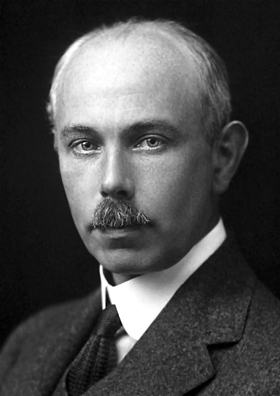
\includegraphics[width=\linewidth]{images/book3/aston.jpg}
\end{minipage}\hspace{0.02\linewidth}%
\begin{minipage}[t]{0.24\linewidth}
\vspace{0pt}
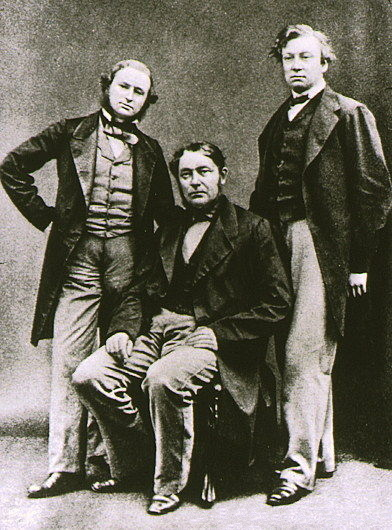
\includegraphics[width=\linewidth]{images/book3/kirchhoff-bunsen.jpg}
\end{minipage}\hfill
\begin{minipage}[t]{0.54\linewidth}
\vspace{0pt}
Gustav Kirchhoff en Robert Bunsen toonden rond 1860 aan dat elk element zijn eigen lijnen geeft in een vlam,
en ontdekten cesium en rubidium aan hun onbekende lijnen. De massaspectrograaf van Francis Aston, vanaf
1919, toonde aan dat de meeste elementen mengsels van isotopen zijn; hij kreeg in 1922 de Nobelprijs voor de Scheikunde.
(Foto's: Aston, onbekende auteur, publiek domein; Kirchhoff, Bunsen en Henry Roscoe in 1862, uit
de collectie van Roscoe, publiek domein; Wikimedia Commons.)
\end{minipage}
\end{history}

\section{Oefeningen}

\begin{exercise}[$\star$]\label{exo:b2:mass-spec-atomic:1}
Geef de $m/z$ van: het \omterm{def:b2:mass-spec-atomic:molecular-ion}{molecuulion} van benzeen \ce{C6H6}; een ion met massa \qty{400}{u} dat twee
ladingen draagt; het geprotoneerde molecuul van cafeïne (\ce{C8H10N4O2}, nominale massa 194) gevormd door elektrospray.
\end{exercise}

\begin{exercise}[$\star$]\label{exo:b2:mass-spec-atomic:2}
Een verbinding van C, H, N en O heeft een \omterm{def:b2:mass-spec-atomic:molecular-ion}{molecuulion} bij $m/z$ 73. Wat kun je zeggen over haar stikstofatomen?
Stel een formule voor.
\end{exercise}

\begin{exercise}[$\star$]\label{exo:b2:mass-spec-atomic:3}
Een groep \omterm{def:b2:mass-spec-atomic:molecular-ion}{molecuulionen} toont twee pieken met twee eenheden ertussen, bijna even hoog. Een andere toont twee
pieken met twee eenheden ertussen in de verhouding 3 : 1. Welke halogenen?
\end{exercise}

\begin{exercise}[$\star$]\label{exo:b2:mass-spec-atomic:4}
Een zout kleurt een vlam geel; een ander karmijnrood. Identificeer de elementen en geef de golflengten van hun
lijnen.
\end{exercise}

\begin{exercise}[$\star\star$]\label{exo:b2:mass-spec-atomic:5}
Een koolwaterstof heeft $M$ bij 100 \% en $M+1$ bij 6.7 \%. Hoeveel koolstofatomen bevat hij?
\end{exercise}

\begin{exercise}[$\star\star$]\label{exo:b2:mass-spec-atomic:6}
Bereken de exacte massa's van \ce{CO}, \ce{N2} en \ce{C2H4} en het oplossend vermogen dat nodig is om
elk paar te scheiden.
\end{exercise}

\begin{exercise}[$\star\star$]\label{exo:b2:mass-spec-atomic:7}
Het EI-spectrum van pentaan-3-on toont pieken bij 86, 57 (\omterm{def:b2:mass-spec-atomic:spectrum}{basispiek}) en 29. Wijs ze toe.
\end{exercise}

\begin{exercise}[$\star\star$]\label{exo:b2:mass-spec-atomic:8}
Het spectrum van pentaan-2-on toont pieken bij 86, 71, 58 en 43 (\omterm{def:b2:mass-spec-atomic:spectrum}{basispiek}). Wijs ze toe, en leg uit
waarom pentaan-3-on slechts een kleine piek bij 58 toont.
\end{exercise}

\begin{exercise}[$\star\star$]\label{exo:b2:mass-spec-atomic:9}
Koperstandaarden bij 1.0, 2.0, 3.0 en \qty{4.0}{mg/L} geven absorbanties 0.052, 0.104, 0.155 en 0.207;
een monster geeft 0.128 (gegevens voor de oefening). Bereken zijn koperconcentratie.
\end{exercise}

\begin{exercise}[$\star\star\star$]\label{exo:b2:mass-spec-atomic:10}
In een vluchttijdanalysator is $L = \qty{1.00}{m}$ en $U = \qty{20.0}{kV}$. Bereken de vluchttijd van
een enkelvoudig geladen ion met massa \qty{1000}{u}, en de tijd die het scheidt van een ion van \qty{1001}{u}.
\end{exercise}

\begin{exercise}[$\star\star\star$]\label{exo:b2:mass-spec-atomic:11}
Bereken de groep \omterm{def:b2:mass-spec-atomic:molecular-ion}{molecuulionen} van dichloormethaan, \ce{CH2Cl2}: waarden van $m/z$ en relatieve
intensiteiten.
\end{exercise}

\begin{exercise}[$\star\star\star$]\label{exo:b2:mass-spec-atomic:12}
Bij ICP-MS interfereert \ce{^{40}Ar^{16}O+} met \ce{^{56}Fe+}. Bereken het oplossend vermogen dat nodig is om
ze te scheiden, en stel een andere uitweg voor.
\end{exercise}

\section{Probleem: een onbekend halogenide}

\begin{problem}[{Weekendprobleem --- een groep molecuulionen met chloor en broom, het aantal
koolstofatomen, de fragmenten, en een structuur die aan elke piek getoetst wordt}]
\label{pb:b2:mass-spec-atomic:1}
Een kleurloze vloeistof, die bij \omterm{def:b2:chromatography:techniques}{gaschromatografie} als één piek elueert, geeft het \omterm{def:b2:mass-spec-atomic:spectrum}{EI-massaspectrum} hieronder (gegevens van het NIST
WebBook). Belangrijkste pieken ($m/z$: relatieve intensiteit): 156: 14.5; 157: 0.5; 158: 18.6; 159: 0.6; 160:
4.4; 107: 6.7; 109: 6.3; 93: 3.3; 95: 2.9; 77: 59; 79: 18.7; 76: 39.5; 49: 12.9; 51: 4.3; 41: 100; 39:
26.2; 27: 24.6. Isotopenabundanties: \ce{^{35}Cl} 0.758, \ce{^{37}Cl} 0.242, \ce{^{79}Br} 0.5069,
\ce{^{81}Br} 0.4931, \ce{^{12}C} 0.989, \ce{^{13}C} 0.011.
% ledger: ms:bromochloropropane, iso:Cl35, iso:Cl37, iso:Br79, iso:Br81, iso:C12, iso:C13, mass:C12, mass:H1, mass:Br79, mass:Cl35

\begin{center}
\begin{tikzpicture}
\begin{axis}[width=0.8\linewidth, height=4.6cm, xmin=20, xmax=170, ymin=0, ymax=112,
  xlabel={$m/z$}, ylabel={relatieve intensiteit}, label style={font=\small},
  tick label style={font=\scriptsize}, ycomb, xtick={27,41,49,77,93,107,122,156}]
\addplot[omDef, thick] table[x=mz, y=I] {figdata/out/bachelor-2-mass-spectra-d.dat};
\end{axis}
\end{tikzpicture}
\end{center}
% figdata: bachelor-2/mass-spectra.py part d

\medskip
\noindent\textbf{Deel I --- Het \omterm{def:b2:mass-spec-atomic:molecular-ion}{molecuulion}.}
\begin{enumerate}
  \item Welke pieken vormen de groep \omterm{def:b2:mass-spec-atomic:molecular-ion}{molecuulionen}? Waarom is het geen enkele piek?
  \item Op welke halogenen wijst een groep van drie pieken met tussenafstand 2?
  \item Wat is de nominale massa van de lichtste isotopische vorm?
  \item Wat zegt de \omterm{def:b2:mass-spec-atomic:nitrogen-rule}{stikstofregel}?
  \item Trek één \ce{^{79}Br} en één \ce{^{35}Cl} af: wat blijft er over, en welk koolwaterstoffragment
        heeft die massa?
  \item Stel een molecuulformule voor en geef haar onverzadigingsgraad.
\end{enumerate}

\medskip
\noindent\textbf{Deel II --- Koolstofatomen en exacte massa.}
\begin{enumerate}[resume]
  \item Schat uit de verhouding 157/156 het aantal koolstofatomen.
  \item Waarom is die schatting hier ruw?
  \item Welke isotopische vormen dragen bij tot de piek bij 158?
  \item Bereken de \omterm{def:b2:mass-spec-atomic:exact-mass}{monoisotopische massa} van het \omterm{def:b2:mass-spec-atomic:molecular-ion}{molecuulion}.
  \item Ook \ce{C10H20O} heeft nominale massa 156 (exact 156.151). Welk oplossend vermogen scheidt de
        twee?
  \item Zou het \omterm{def:b2:mass-spec-atomic:molecular-ion}{molecuulion} van een verbinding met een binding C=C en dezelfde halogenen een andere
        nominale massa hebben?
\end{enumerate}

\medskip
\noindent\textbf{Deel III --- Fragmenten.}
\begin{enumerate}[resume]
  \item Het paar 77/79 staat in de verhouding 3 : 1. Welk atoom is verloren gegaan, en wat is het ion?
  \item Verklaar de piek bij 76.
  \item Wijs de \omterm{def:b2:mass-spec-atomic:spectrum}{basispiek} bij 41 toe.
  \item Wijs het paar 49/51 toe.
  \item Wijs de paren 93/95 en 107/109 toe.
  \item Waarom gaat een broomatoom gemakkelijker verloren dan een chlooratoom?
  \item 1-Broom-1-chloorpropaan zou \ce{CHBrCl+} geven bij 127, 129 en 131. Ondersteunt het spectrum dat?
\end{enumerate}

\medskip
\noindent\textbf{Deel IV --- De structuur.}
\begin{enumerate}[resume]
  \item Stel de structuur voor.
  \item Controleer dat ze elke vermelde piek verklaart.
  \item Kan er een \omterm{def:b2:mass-spec-atomic:fragmentation}{omlegging van McLafferty} optreden? Waarom?
  \item Teken het isomeer dat een sterke piek bij $m/z$ 63/65 zou geven en geen bij 49/51.
  \item Welke isotopische vormen maken de piek bij 160?
  \item Bereken uit de isotopenabundanties de verhouding van de pieken $M$, $M+2$ en $M+4$ voor één
        chlooratoom en één broomatoom, en vergelijk ze met het spectrum.
\end{enumerate}
\end{problem}
